\documentclass[12pt,a4paper]{article}
\usepackage[utf8]{inputenc}
\usepackage[italian]{babel}
\usepackage[T1]{fontenc}
\usepackage{lmodern} % O usa 'times' per un font più simile al PDF
\usepackage{geometry}
\geometry{margin=3cm}
\usepackage{graphicx}
\usepackage{fancyhdr}
\usepackage{setspace}
\usepackage{titlesec}
\usepackage{caption}
\usepackage{booktabs}
\usepackage{float}
\usepackage{hyperref}
\graphicspath{ {./images/} }
\pagestyle{plain}
\onehalfspacing % Interlinea 1.5
\setlength{\parskip}{0.5em}

% ------------------ FRONTESPIZIO ------------------
\begin{document}
\begin{titlepage}
    \centering
    {\scshape\LARGE Università degli Studi di Padova \par}
    \vspace{1cm}
    {\scshape\Large Corso di Laurea in Informatica \par}
    \vspace{3cm}
    {\Huge\bfseries Basi di Dati per un Sistema di gestione di Serie TV in Streaming \par}
    \vspace{2cm}
    {\Large Gruppo: Ceron Tommaso, Parolin Dennis\par}
    \vfill
    {\large Anno Accademico 2024/2025\par}
\end{titlepage}

% ------------------ INDICE (se necessario) ------------------
% \tableofcontents
% \newpage

% ------------------ CONTENUTO ------------------

\section{Abstract}
Questo progetto sviluppa una base di dati per gestire delle serie tv, composte da stagioni ed episodi, e dai loro attori e registi. Inoltre, questa base di dati permette di gestire degli utenti e gli episodi che guardano, ai quali possono dare un voto.\newline L’obbiettivo principale è quello di gestire la struttura delle serie tv, gestire le relazioni di quest’ ultime con il cast e il regista che vi partecipa e infine registrare ciò che un utente guarda.\newline
La base di dati distingue le persone in utenti, registi e attori, ognuno con degli attributi e relazioni distinte.\newline
Una serie si compone di almeno una stagione, che a sua volta è composta da almeno un episodio. Opzionalmente una Serie TV può anche contenere una Opening (ovvero una sigla iniziale).\newline
Infine, il sistema tiene traccia delle piattaforme di streaming che mettono a disposizione una determinata serie tv, e degli utenti che sottoscrivono un abbonamento con uno o più di queste piattaforme. \newline

\section{Analisi dei Requisiti}
In questa sezione riassumiamo i requisiti che caratterizzano la base di dati.\newline\newline
\textbf{Serie TV.} Una serie TV è identificata da un titolo e un anno e contiene questi attributi:
\begin{itemize}
  \item Titolo
  \item Anno di Inizio
  \item Descrizione
  \item Genere
\end{itemize}
Una Serie TV è composta da una o più stagioni, e da zero o una Opening (sigla iniziale) \newline\newline\newline\newline
\textbf{Stagioni.} Una stagione è identificata da un identificatore univoco e contiene questi attributi:
\begin{itemize}
    \item Identificatore
    \item Numero
    \item Anno
\end{itemize}
Una stagione è composta da uno o più episodi\newline\newline
\textbf{Episodio.} Un episodio è identificato da un identificatore univoco e contiene questi attributi:
\begin{itemize}
    \item Identificatore
    \item Numero
    \item Durata (in minuti)
    \item Titolo
    \item Numero di utenti (che hanno guardato l' episodio)
\end{itemize}
\textbf{Opening.} Una opening è identificata da un titolo, e contiene questi attributi:
\begin{itemize}
    \item Titolo
    \item Compositore
    \item Durata
\end{itemize}
\textbf{Persona.} Una persona generica è identificata da un identificatore univoco e contiene i seguenti attributi: 
\begin{itemize}
    \item Identificatore
    \item Nome
    \item Data di nascita
\end{itemize}
Una persona si suddivide in \textbf{Utente}, \textbf{Nome} e \textbf{Registi}\newpage
\textbf{Utenti.} Un utente, oltre agli attributi di \textit{Persona} contiene:
\begin{itemize}
    \item Username
    \item Email
\end{itemize}
\textbf{Attore.} Un attore, oltre agli attributi di \textit{Persona}, contiene:
\begin{itemize}
    \item Nazionalita'
    \item Il numero di film in cui ha partecipato
\end{itemize}
\textbf{Regista.} Un regista, oltre agli attributi di \textit{Persona}, contiene:
\begin{itemize}
    \item Nazionalita
    \item Il genere di film creati
\end{itemize}
\textbf{Piattaforma streaming.} Una piattaforma streaming e' identificata dal suo nome e contiene i seguenti attributi:
\begin{itemize}
    \item Nome 
    \item Costo mensile
\end{itemize}
\section{Progettazione concettuale}
\subsection{Lista entità}
Il database si compone delle seguenti entità:
\begin{itemize}
    \item \textbf{SerieTV:} Rappresenta una Serie Tv univoca, con una o più stagioni.
    \begin{itemize}
        \item \underline{Titolo}: string
        \item \underline{AnnoInizio} (ovvero l'anno della prima stagione): int
        \item Genere: string
        \item Descrizione: string
    \end{itemize}
    \item \textbf{Stagione:} Rappresenta una stagione di una specifica Serie Tv
    \begin{itemize}
        \item \underline{Numero\_ stagione}: int
        \item Anno: int
    \end{itemize}
    \item \textbf{Episodio:} Rappresenta un singolo episodio di una specifica stagione
    \begin{itemize}
        \item \underline{Numero\_ episodio}: int
        \item Durata (in minuti): int
        \item Titolo: string
        \item Numero\_utenti (che hanno guardato l'episodio): int
    \end{itemize}
    \item \textbf{Opening:} Rappresenta la sigla iniziale di una SerieTv, se presente.
    \begin{itemize}
        \item \underline{Titolo}: string
        \item Durata: int
        \item Compositore: string
    \end{itemize}
    \item \textbf{Persona:} Rappresenta una persona generica.
    \begin{itemize}
        \item \underline{Identificatore}: int
        \item Nome: string
        \item Data\_ nascita: date
    \end{itemize}
    \item \textbf{Utente:} Rappresenta una specializzazione di Persona, rappresenta un abbonato a una o più piattaforme streaming
    \begin{itemize}
        \item Username: string
        \item Email: string
    \end{itemize}
    \item \textbf{Attore:} Rappresenta una specializzazione di Persona, partecipa a una o più serie TV.
    \begin{itemize}
        \item Nazionalita': string
        \item Numero\_serie (in cui ha partecipato): int
    \end{itemize}
    \item \textbf{Regista:} Rappresenta una specializzazione di Persona, ha diretto una o più serie TV.
    \begin{itemize}
        \item Nazionalita: string
        \item Genere\_serie: string
    \end{itemize}
    \item \textbf{Piattaforma streaming:} Rappresenta una piattaforma che contiene una o più serie Tv, e a cui gli utenti possono abbonarsi con vari tipi di abbonamento.
    \begin{itemize}
        \item \underline{Nome}: string
        \item Costo\_mensile: float
    \end{itemize}
\end{itemize}
\subsection{Lista relazioni}
\begin{itemize}
    \item Serie TV-> (1, N) ->ComposizioneStag<-(1,1) <-Stagione 
    \begin{itemize}
        \item Una Serie Tv è composta da una o più stagioni
        \item Una stagione compone una sola Serie Tv 
    \end{itemize}
    \item Stagione-> (1, N) ->ComposizioneEP<-(1,1) <-Episodio
    \begin{itemize}
        \item Una stagione è composta da uno o più episodi
        \item Un episodio compone una sola stagione
    \end{itemize}
    \item Serie TV-> (1,1) ->Contenimento<-(1, N) <-Piattaforma-Streaming
    \begin{itemize}
        \item Una Serie Tv è contenuta (può essere vista) in una sola piattaforma streaming
        \item Una piattaforma streaming può contenere una o più serie tv 
    \end{itemize}
    \item Piattaforma-Streaming (1, N) ->Sottoscrizione<-(1, N) <-Utente
    \begin{itemize}
        \item Ad una piattaforma streaming si sottoscrivono uno o più utenti
        \item Un utente può sottoscriversi a una o più piattaforme streaming (minimo una per essere considerato utente)
        \item Questa relazione contiene i seguenti attributi:
        \begin{itemize}
            \item Data\_inizio: date
            \item Data\_fine: date
            \item Tpo\_abbonamento: string
        \end{itemize}
    \end{itemize}
    \item Utente-> (0, N) ->Visiona<-(0, N) <-Episodio
    \item \begin{itemize}
        \item Un utente può vedere 0 o più episodi di stagioni differenti
        \item Un episodio generico può essere visto da nessuno o da più utenti
        \item Questa relazione contiene i seguenti attributi:
        \begin{itemize}
            \item Data: date
            \item Voto: int
        \end{itemize}
        Il voto e' opzionale.
    \end{itemize}
    \begin{itemize}
        \item Serie TV-> (1, N) ->RecitaIn<-(1, N) <-Attore
        \begin{itemize}
            \item In una serie tv recitano uno o più attori
            \item Un attore può recitare in una o più sere tv
            \item Questa relazione contiene i seguenti attributi:
            \begin{itemize}
                \item Ruolo: string
            \end{itemize}
        \end{itemize}
    \end{itemize}
    \item Serie TV-> (1,1) ->Direzione<-(1, N)<-Regista 
    \begin{itemize}
        \item Una serie tv è diretta da un solo regista 
        \item Un regista può dirigere una o più serie 
    \end{itemize}
    \item Serie Tv-> (0,1) ->ContenimentoOpening<-(1,1)<-Opening
    \begin{itemize}
        \item Una serie tv contiene zero o una opening
        \item Una opening appartiene a una sola Serie Tv 
    \end{itemize} 
\end{itemize}
\subsection{Lista generalizzazioni}
\textbf{Persona} è una generalizzazione totale di \textbf{UTENTE}, \textbf{ATTORE} e \textbf{REGISTA} 
\subsection{Schema E-R}
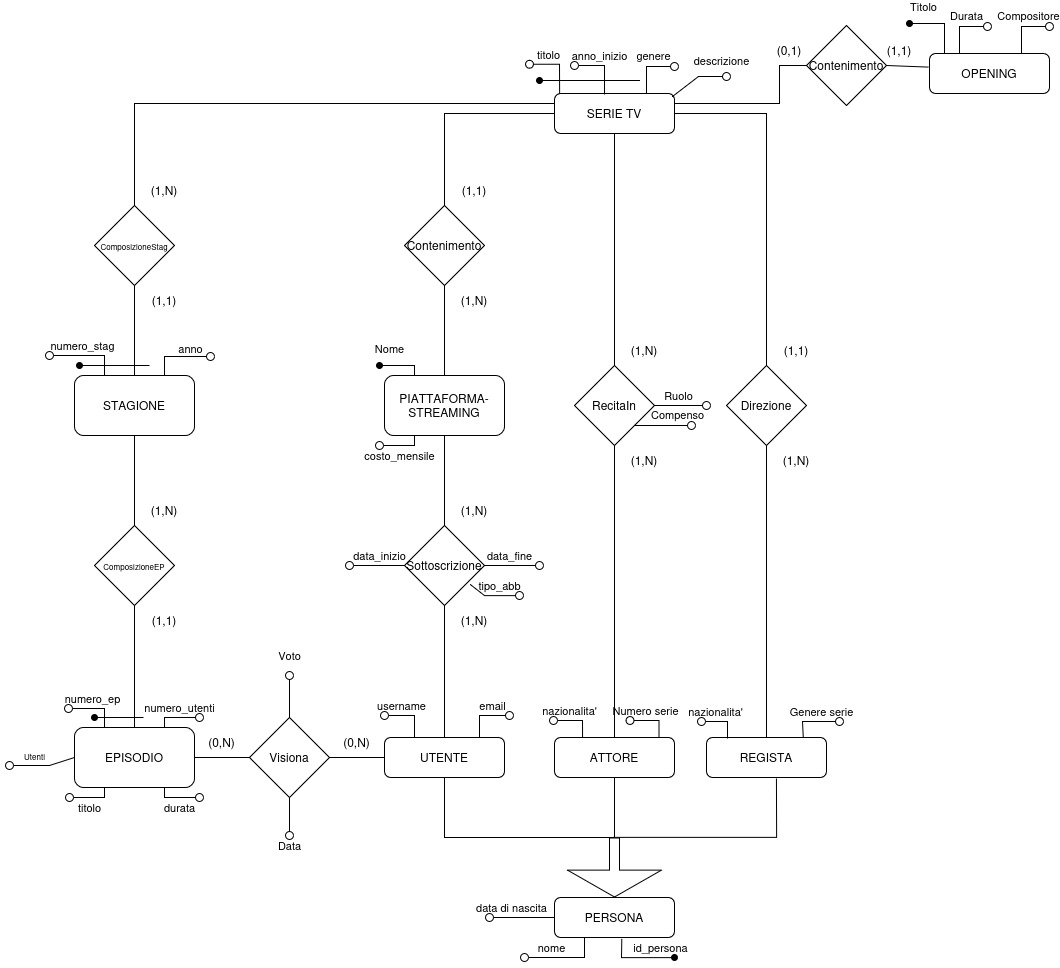
\includegraphics[scale=0.45]{schema-no-ristrutt}
\section{Progettazione Logica}
In questa sezione illustriamo la traduzione dello schema concettuale in schema logico, per rappresentare i dati nel modo piu' efficace possibile. 
Andiamo quindi ad analizzare le ridondanze, per comprendere se sia preferibile eliminarle o mantenerle. 
Procediamo poi con l'eliminazione delle generalizzazioni e infine mostriamo lo schema ristrutturato.
\subsection{Analisi delle ridondanze}
\subsubsection{Ridondanza "NumeroSerieTv"}
Possiamo notare che attributo “Numero Serie Tv” del sottoinsieme “Attore” entità “Persona” può essere calcolato dalla relazione RecitaIn, poiché è il conteggio di tutte le Serie Tv per quel determinato attore.
Questo attributo viene modificato (almeno una volta) ogni volta che viene inserita una nuova SerieTv (stimiamo circa 5 nuovi inserimenti al giorno)
e viene visualizzato ogni volta un utente vuole sapere in quanti film ha recitato un attore (stimiamo 25 al giorno).
Il tutto si riassume nelle seguenti operazioni:
\begin{itemize}
    \item \textbf{Operazione 1 (5 al giorno)}: inserimento di una nuova tupla in RecitaIn
    \item \textbf{Operazione 2 (25 al giorno)}: Visualizzare in quanti film ha recitato un attore.
\end{itemize}

Assumiamo i seguenti dati:
\begin{center}
\begin{tabular}{|c c c|} 
 \hline
 Concetto & Costrutto & Volume \\ [0.5ex] 
 \hline\hline
 Attore & Entità  & 1000\\ 
 \hline
 RecitaIn & Relazione & 2000\\[1ex] 
 \hline
\end{tabular}
\end{center}
\textbf{Con Ridondanza}
\begin{itemize}
    \item Operazione 1
    \begin{center}
    \begin{tabular}{|c c c c|} 
    \hline
    Concetto & Costrutto & Accessi & Tipo \\ [0.5ex] 
    \hline\hline
    SerieTv & Entità  & 1 & S\\
    \hline
    RecitaIn & Relazione & 1 & S\\
    \hline
    Attore & Entità & 1 & L\\
    \hline
    Attore & Entità & 1 & S\\[1ex]
    \hline
    \end{tabular}
    \end{center}
\end{itemize}

% Aggiungi altre sezioni qui...

\end{document}
